% This is a template for Ph.D. dissertations in the UCI format.
% 
% All fonts, including those for sub- and superscripts, must be 10
% points or larger.  Recommended sizes are 14-point for chapter
% headings, 12-point for the main body of text and figure/table
% titles, and 10-point for footnotes, sub- and super-scripts, and text
% in figures and tables.
%
% Notes: Add short title to figures, sections, via square brackets,
% e.g. \section[short]{long}.
%
\documentclass[12pt,fleqn]{ucithesis}

% A few common packages
\usepackage{amsmath}
\usepackage{amsthm}
\usepackage{array}
\usepackage{graphicx}
\usepackage{natbib}
\usepackage{relsize}
\usepackage[titletoc]{appendix}

% Some other useful packages
\usepackage{caption}
\usepackage{subcaption}  % \begin{subfigure}...\end{subfigure} within figure
\usepackage{multirow}
\usepackage{tabularx}
\usepackage{longtable}
\usepackage{float}
\usepackage{wrapfig}
\usepackage{parskip}
\usepackage{amssymb}
% uncomment the following to accommodate non-English language characters:
%\usepackage[T1]{fontenc}

\usepackage{lipsum} % for dummy text; REMOVE

% Uncomment the following to attempt to enforce Type 1 or TrueType 
% fonts. ProQuest does not want the type 3 fonts used by default as
% of Dec. 2019 - see 
% https://support.proquest.com/articledetail?id=kA01W000000k9o2SAA . 
% If you are unable to embed fonts such as 'Zapf Dingbats' or 
% 'Symbol', try using raster images (.jpg or .png) instead of vector 
%images (.pdf or .eps).
% \usepackage[T1]{fontenc} 

% plainpages=false fixes the "duplicate ignored" error with page counters
% Set pdfborder to 0 0 0 to disable colored borders around PDF hyperlinks
\usepackage[plainpages=false,pdfborder={0 0 0}]{hyperref}

% Uncomment the following line to use the algorithm package,
% which provides an algorithm environment similar to figure and table
% ("\begin{algorithm}...\end{algorithm}"). A list of algorithms will
% automatically be added in the preliminary pages. Note that you
% probably want a package for the actual code to go with this (e.g.,
% algorithmic).
%\usepackage{algorithm}

% Uncomment the following line to enable Unicode support. This will allow you
% to enter non-ASCII characters (such as accented characters) directly without
% having to use LaTeX's awkward escape syntax (e.g., \'{e})
% NOTE: You may have to install the ucs.sty package for this to work. See:
% http://www.unruh.de/DniQ/latex/unicode/
%\usepackage[utf8x]{inputenc}

% Uncomment the following to avoid "widowing", where page breaks cause
% single lines of paragraphs to float onto the next page (this is not
% a UCI requirement but more of an aesthetic choice).
%\widowpenalty=10000
%\clubpenalty=10000

% Modify or extend these at will.
\newtheorem{theorem}{\textsc{Theorem}}[chapter]
\newtheorem{definition}{\textsc{Definition}}[chapter]
\newtheorem{example}{\textsc{Example}}[chapter]

% Macros for title, author, abstract, etc.
% This information can be edited in the file preliminaries.tex
% THis file is incorporated into the main file by inserting the command \preliminarypages on its own line in "thesis.tex"
% ######################################################### % 
% #################    THESIS TITLE    #################### % 
% ######################################################### % 
% The title of your thesis. This should be the same title as appears on your advancement/defense announcement
\thesistitle{YOUR THESIS TITLE HERE}

%"Dissertation" for PhD, "Thesis" for master's
\documenttitle{Thesis}

% ######################################################### % 
% #################    DEGREE FIELD    #################### % 
% ######################################################### % 
% Comment out for PhD Thesis; Uncomment for Masters Thesis
\degreename{Master of Science}

% Comment out for Masters Thesis; Uncomment for PhD Thesis
% \degreename{Master of Science}


% Use the wording given in the official list of degrees awarded by UCI:
% http://www.rgs.uci.edu/grad/academic/degrees_offered.htm
\degreefield{YOUR DEGREE FIELD}

% ######################################################### % 
% #################     YOUR NAME      #################### % 
% ######################################################### % 
% Your name as it appears on official UCI records.
\authorname{YOUR NAME HERE}


% ######################################################### % 
% ###############   THESIS COMMITTEE   #################### % 
% ######################################################### % 
% Use the full name of each committee member and full title 
% (e.g. Professor/Associate Professor).
\committeechair{Professor <CHAIR: NAME HERE>}
\othercommitteemembers
{
  Associate Professor NAME HERE \\
  Assistant Professor NAME HERE
}



% ######################################################### % 
% #################     COPYRIGHT      #################### % 
% ######################################################### % 
\degreeyear{2021}

\copyrightdeclaration
{
  {\copyright} {\Degreeyear} \Authorname
}


% ######################################################### % 
% ##############  PREVIOUS PUBLICATIONS   ################# % 
% ######################################################### % 
% If you have previously published parts of your manuscript, you must list the
% copyright holders; see Section 3.2 of the UCI Thesis and Dissertation Manual.
% Otherwise, this section may be omitted.
% \prepublishedcopyrightdeclaration
% {
% 	Chapter 4 {\copyright} 2003 Springer-Verlag \\
% 	Portion of Chapter 5 {\copyright} 1999 John Wiley \& Sons, Inc. \\
% 	All other materials {\copyright} {\Degreeyear} \Authorname
% }



% ######################################################### % 
% ###########  DEDICATION & ACKNOWLEDGEMENTS  ############# % 
% ######################################################### % 
% The dedication page is optional
% (comment out to exclude).
\dedications
{
  (Optional dedication page)
  
  To ...
}

\acknowledgments
{
  I would like to thank...
  
  (You must acknowledge grants and other funding assistance. 
  
  You may also acknowledge the contributions of professors and
  friends.
  
  You also need to acknowledge any publishers of your previous
  work who have given you permission to incorporate that work
  into your dissertation. See Section 3.2 of the UCI Thesis and
  Dissertation Manual.)
}



% ######################################################### % 
% #################   CUSTOM COMMANDS  #################### % 
% ######################################################### % 
% Some custom commands for your list of publications and software.
\newcommand{\mypubentry}[3]{
  \begin{tabular*}{1\textwidth}{@{\extracolsep{\fill}}p{4.5in}r}
    \textbf{#1} & \textbf{#2} \\ 
    \multicolumn{2}{@{\extracolsep{\fill}}p{.95\textwidth}}{#3}\vspace{6pt} \\
  \end{tabular*}
}
\newcommand{\mysoftentry}[3]{
  \begin{tabular*}{1\textwidth}{@{\extracolsep{\fill}}lr}
    \textbf{#1} & \url{#2} \\
    \multicolumn{2}{@{\extracolsep{\fill}}p{.95\textwidth}}
    {\emph{#3}}\vspace{-6pt} \\
  \end{tabular*}
}


% ######################################################### % 
% #################   CV (PhD Only)    #################### % 
% ######################################################### % 

% CV is required for PhD theses, but not Master's
% comment out to exclude

% Include, at minimum, a listing of your degrees and educational
% achievements with dates and the school where the degrees were
% earned. This should include the degree currently being
% attained. Other than that it's mostly up to you what to include here
% and how to format it, below is just an example.
%

% \curriculumvitae
% {

% \textbf{EDUCATION}
  
%   \begin{tabular*}{1\textwidth}{@{\extracolsep{\fill}}lr}
%     \textbf{Doctor of Philosophy in Computer Science} & \textbf{2012} \\
%     \vspace{6pt}
%     University name & \emph{City, State} \\
%     \textbf{Bachelor of Science in Computational Sciences} & \textbf{2007} \\
%     \vspace{6pt}
%     Another university name & \emph{City, State} \\
%   \end{tabular*}

% \vspace{12pt}
% \textbf{RESEARCH EXPERIENCE}

%   \begin{tabular*}{1\textwidth}{@{\extracolsep{\fill}}lr}
%     \textbf{Graduate Research Assistant} & \textbf{2007--2012} \\
%     \vspace{6pt}
%     University of California, Irvine & \emph{Irvine, California} \\
%   \end{tabular*}

% \vspace{12pt}
% \textbf{TEACHING EXPERIENCE}

%   \begin{tabular*}{1\textwidth}{@{\extracolsep{\fill}}lr}
%     \textbf{Teaching Assistant} & \textbf{2009--2010} \\
%     \vspace{6pt}
%     University name & \emph{City, State} \\
%   \end{tabular*}

% \pagebreak

% \textbf{REFEREED JOURNAL PUBLICATIONS}

%   \mypubentry{Ground-breaking article}{2012}{Journal name}

% \vspace{12pt}
% \textbf{REFEREED CONFERENCE PUBLICATIONS}

%   \mypubentry{Awesome paper}{Jun 2011}{Conference name}
%   \mypubentry{Another awesome paper}{Aug 2012}{Conference name}

% \vspace{12pt}
% \textbf{SOFTWARE}

%   \mysoftentry{Magical tool}{http://your.url.here/}
%   {C++ algorithm that solves TSP in polynomial time.}

% }

% The abstract was previously limited to a maximum of 350 words, 
% but the UCI manual at https://etd.lib.uci.edu/electronic/td2e#2.2.1.
% currently does not indicate that there is any word limit for the abstract
\thesisabstract
{
Your abstract goes here \\
NOTE: the maximum word count for the thesis abstract is 250 words.
}


%%% Local Variables: ***
%%% mode: latex ***
%%% TeX-master: "thesis.tex" ***
%%% End: ***


% Add PDF document info fields
\hypersetup{
	pdftitle={\Thesistitle},
	pdfauthor={\Authorname},
	pdfsubject={\Degreefield},
}

% Uncomment the following to have numbered subsubsections (by default
% numbering goes only to subsections).
%\setcounter{secnumdepth}{4}


% Set this to only select a subset of the includes directives below.
% Very handy to speed up compilation if you're working on a certain
% part of your thesis. It conserves page numbers, references, etc.
% even for non-included files.
%\includeonly{chapter1}

\begin{document}


% ######################################################### % 
% #################  PRELIMINARIES     #################### % 
% ######################################################### % 
% These pages can be edited in the file "preliminaries.tex"
% Preliminary pages are always loaded (TOC, CV, etc.)
\preliminarypages

% ######################################################### % 
% #################     YOUR NAME      #################### % 
% ######################################################### % 
% Include the different components of your thesis, in separate files.
% Using \include allows you to set \includeonly above.
\chapter{Introduction}

%%%%%%%%%%%%%%%%%%%%%%%%%%%%%%%%%%%%%%%%%%%%%%%%%%%%%%%%%%%%%%%%%%%%%%%%%
%%%%%%%%%%%%%%%%%%%%% SECTION NAME %%%%%%%%%%%%%%%%%%%%%%%%%%%%%%%%%%%%%%
%%%%%%%%%%%%%%%%%%%%%%%%%%%%%%%%%%%%%%%%%%%%%%%%%%%%%%%%%%%%%%%%%%%%%%%%%
\section{SECTION NAME}
\begin{figure}
    \centering
    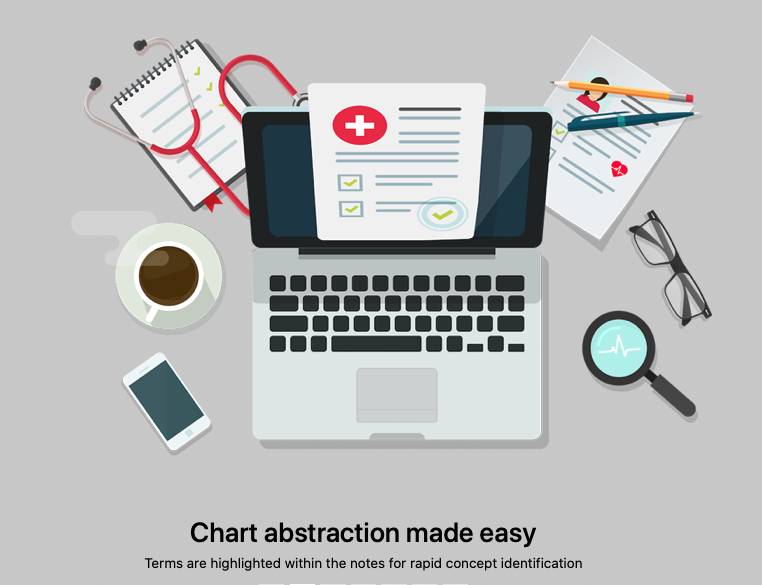
\includegraphics[width=0.8\linewidth]{Resources/Images/Banner1.png}
    \caption{An example figure for an opening graphic}
    \label{fig:emerse_banner1}
\end{figure}

This chapter is your introduction. Depending on your writing style, field of work, and project, you may choose to combine this into one chapter with the \texttt{\textbf{"Background"}} chapter.

This chapter is incorporated into the main body of writing by entering the following line(s) of command(s) in \texttt{thesis.tex}
\begin{verbatim}
# this line goes in the file "thesis.tex"
\chapter{Introduction}

%%%%%%%%%%%%%%%%%%%%%%%%%%%%%%%%%%%%%%%%%%%%%%%%%%%%%%%%%%%%%%%%%%%%%%%%%
%%%%%%%%%%%%%%%%%%%%% SECTION NAME %%%%%%%%%%%%%%%%%%%%%%%%%%%%%%%%%%%%%%
%%%%%%%%%%%%%%%%%%%%%%%%%%%%%%%%%%%%%%%%%%%%%%%%%%%%%%%%%%%%%%%%%%%%%%%%%
\section{SECTION NAME}
\begin{figure}
    \centering
    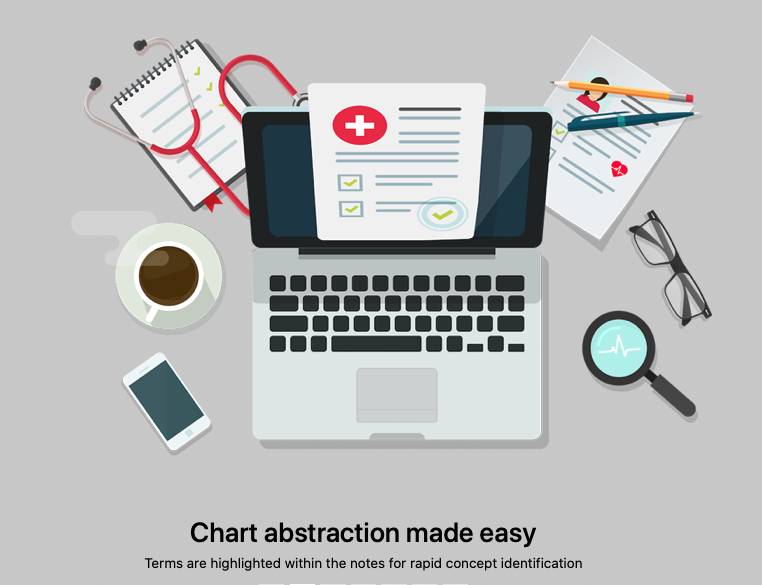
\includegraphics[width=0.8\linewidth]{Resources/Images/Banner1.png}
    \caption{An example figure for an opening graphic}
    \label{fig:emerse_banner1}
\end{figure}

This chapter is your introduction. Depending on your writing style, field of work, and project, you may choose to combine this into one chapter with the \texttt{\textbf{"Background"}} chapter.

This chapter is incorporated into the main body of writing by entering the following line(s) of command(s) in \texttt{thesis.tex}
\begin{verbatim}
# this line goes in the file "thesis.tex"
\chapter{Introduction}

%%%%%%%%%%%%%%%%%%%%%%%%%%%%%%%%%%%%%%%%%%%%%%%%%%%%%%%%%%%%%%%%%%%%%%%%%
%%%%%%%%%%%%%%%%%%%%% SECTION NAME %%%%%%%%%%%%%%%%%%%%%%%%%%%%%%%%%%%%%%
%%%%%%%%%%%%%%%%%%%%%%%%%%%%%%%%%%%%%%%%%%%%%%%%%%%%%%%%%%%%%%%%%%%%%%%%%
\section{SECTION NAME}
\begin{figure}
    \centering
    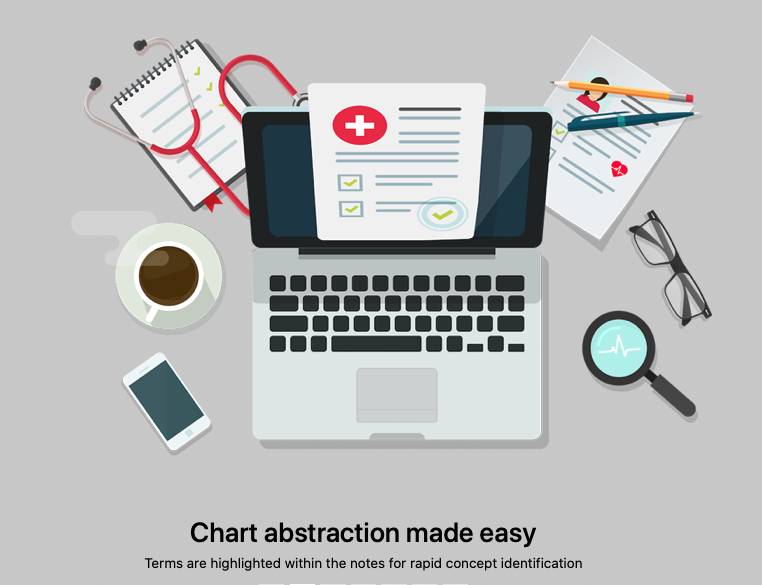
\includegraphics[width=0.8\linewidth]{Resources/Images/Banner1.png}
    \caption{An example figure for an opening graphic}
    \label{fig:emerse_banner1}
\end{figure}

This chapter is your introduction. Depending on your writing style, field of work, and project, you may choose to combine this into one chapter with the \texttt{\textbf{"Background"}} chapter.

This chapter is incorporated into the main body of writing by entering the following line(s) of command(s) in \texttt{thesis.tex}
\begin{verbatim}
# this line goes in the file "thesis.tex"
\include{Chapters/chapter1}
\end{verbatim}



%%% Local Variables: ***
%%% mode: latex ***
%%% TeX-master: "thesis.tex" ***
%%% End: ***

\end{verbatim}



%%% Local Variables: ***
%%% mode: latex ***
%%% TeX-master: "thesis.tex" ***
%%% End: ***

\end{verbatim}



%%% Local Variables: ***
%%% mode: latex ***
%%% TeX-master: "thesis.tex" ***
%%% End: ***

\chapter{Background \& Literature}

%%%%%%%%%%%%%%%%%%%%%%%%%%%%%%%%%%%%%%%%%%%%%%%%%%%%%%%%%%%%%%%%%%%%%%%%%
%%%%%%%%%%%%%%%%%%%%% SECTION NAME %%%%%%%%%%%%%%%%%%%%%%%%%%%%%%%%%%%%%%
%%%%%%%%%%%%%%%%%%%%%%%%%%%%%%%%%%%%%%%%%%%%%%%%%%%%%%%%%%%%%%%%%%%%%%%%%
\section{SECTION NAME}

This chapter is your background and literature review. Depending on your writing style, field of work, and project, you may choose to combine this into one chapter with the \texttt{\textbf{"Introduction"}} chapter.

This chapter is incorporated into the main body of writing by entering the following line(s) of command(s) in \texttt{thesis.tex}
\begin{verbatim}
# this line goes in the file "thesis.tex"
\chapter{Background \& Literature}

%%%%%%%%%%%%%%%%%%%%%%%%%%%%%%%%%%%%%%%%%%%%%%%%%%%%%%%%%%%%%%%%%%%%%%%%%
%%%%%%%%%%%%%%%%%%%%% SECTION NAME %%%%%%%%%%%%%%%%%%%%%%%%%%%%%%%%%%%%%%
%%%%%%%%%%%%%%%%%%%%%%%%%%%%%%%%%%%%%%%%%%%%%%%%%%%%%%%%%%%%%%%%%%%%%%%%%
\section{SECTION NAME}

This chapter is your background and literature review. Depending on your writing style, field of work, and project, you may choose to combine this into one chapter with the \texttt{\textbf{"Introduction"}} chapter.

This chapter is incorporated into the main body of writing by entering the following line(s) of command(s) in \texttt{thesis.tex}
\begin{verbatim}
# this line goes in the file "thesis.tex"
\chapter{Background \& Literature}

%%%%%%%%%%%%%%%%%%%%%%%%%%%%%%%%%%%%%%%%%%%%%%%%%%%%%%%%%%%%%%%%%%%%%%%%%
%%%%%%%%%%%%%%%%%%%%% SECTION NAME %%%%%%%%%%%%%%%%%%%%%%%%%%%%%%%%%%%%%%
%%%%%%%%%%%%%%%%%%%%%%%%%%%%%%%%%%%%%%%%%%%%%%%%%%%%%%%%%%%%%%%%%%%%%%%%%
\section{SECTION NAME}

This chapter is your background and literature review. Depending on your writing style, field of work, and project, you may choose to combine this into one chapter with the \texttt{\textbf{"Introduction"}} chapter.

This chapter is incorporated into the main body of writing by entering the following line(s) of command(s) in \texttt{thesis.tex}
\begin{verbatim}
# this line goes in the file "thesis.tex"
\include{Chapters/chapter2}
\end{verbatim}



%%% Local Variables: ***
%%% mode: latex ***
%%% TeX-master: "thesis.tex" ***
%%% End: ***

\end{verbatim}



%%% Local Variables: ***
%%% mode: latex ***
%%% TeX-master: "thesis.tex" ***
%%% End: ***

\end{verbatim}



%%% Local Variables: ***
%%% mode: latex ***
%%% TeX-master: "thesis.tex" ***
%%% End: ***

\chapter{Methods}
This chapter is incorporated into the main body of writing by entering the following line(s) of command(s) in \texttt{thesis.tex}
\begin{verbatim}
# this line goes in the file "thesis.tex"
\chapter{Methods}
This chapter is incorporated into the main body of writing by entering the following line(s) of command(s) in \texttt{thesis.tex}
\begin{verbatim}
# this line goes in the file "thesis.tex"
\chapter{Methods}
This chapter is incorporated into the main body of writing by entering the following line(s) of command(s) in \texttt{thesis.tex}
\begin{verbatim}
# this line goes in the file "thesis.tex"
\include{Chapters/chapter3}
\end{verbatim}

%%%%%%%%%%%%%%%%%%%%%%%%%%%%%%%%%%%%%%%%%%%%%%%%%%%%%%%%%%%%%%%%%%%%%%%%%
%%%%%%%%%%%%%%%%%%%%% RECRUITMENT %%%%%%%%%%%%%%%%%%%%%%%%%%%%%%%%%%%%%%%
%%%%%%%%%%%%%%%%%%%%%%%%%%%%%%%%%%%%%%%%%%%%%%%%%%%%%%%%%%%%%%%%%%%%%%%%%
\section{Recruitment}


%%%%%%%%%%%%%%%%%%%%%%%%%%%%%%%%%%%%%%%%%%%%%%%%%%%%%%%%%%%%%%%%%%%%%%%%%
%%%%%%%%%%%%%%%%%%%%% DATA COLLECTION %%%%%%%%%%%%%%%%%%%%%%%%%%%%%%%%%%%
%%%%%%%%%%%%%%%%%%%%%%%%%%%%%%%%%%%%%%%%%%%%%%%%%%%%%%%%%%%%%%%%%%%%%%%%%
\section{Data Collection}



%%%%%%%%%%%%%%%%%%%%%%%%%%%%%%%%%%%%%%%%%%%%%%%%%%%%%%%%%%%%%%%%%%%%%%%%%
%%%%%%%%%%%%%%%%%%%% DATA ANALYSIS %%%%%%%%%%%%%%%%%%%%%%%%%%%%%%%%%%%%%%
%%%%%%%%%%%%%%%%%%%%%%%%%%%%%%%%%%%%%%%%%%%%%%%%%%%%%%%%%%%%%%%%%%%%%%%%%
\section{Data Analysis}
\subsection{Qualitative Analysis}
\subsection{Quantitative Analysis}


%%% Local Variables: ***
%%% mode: latex ***
%%% TeX-master: "thesis.tex" ***
%%% End: ***

\end{verbatim}

%%%%%%%%%%%%%%%%%%%%%%%%%%%%%%%%%%%%%%%%%%%%%%%%%%%%%%%%%%%%%%%%%%%%%%%%%
%%%%%%%%%%%%%%%%%%%%% RECRUITMENT %%%%%%%%%%%%%%%%%%%%%%%%%%%%%%%%%%%%%%%
%%%%%%%%%%%%%%%%%%%%%%%%%%%%%%%%%%%%%%%%%%%%%%%%%%%%%%%%%%%%%%%%%%%%%%%%%
\section{Recruitment}


%%%%%%%%%%%%%%%%%%%%%%%%%%%%%%%%%%%%%%%%%%%%%%%%%%%%%%%%%%%%%%%%%%%%%%%%%
%%%%%%%%%%%%%%%%%%%%% DATA COLLECTION %%%%%%%%%%%%%%%%%%%%%%%%%%%%%%%%%%%
%%%%%%%%%%%%%%%%%%%%%%%%%%%%%%%%%%%%%%%%%%%%%%%%%%%%%%%%%%%%%%%%%%%%%%%%%
\section{Data Collection}



%%%%%%%%%%%%%%%%%%%%%%%%%%%%%%%%%%%%%%%%%%%%%%%%%%%%%%%%%%%%%%%%%%%%%%%%%
%%%%%%%%%%%%%%%%%%%% DATA ANALYSIS %%%%%%%%%%%%%%%%%%%%%%%%%%%%%%%%%%%%%%
%%%%%%%%%%%%%%%%%%%%%%%%%%%%%%%%%%%%%%%%%%%%%%%%%%%%%%%%%%%%%%%%%%%%%%%%%
\section{Data Analysis}
\subsection{Qualitative Analysis}
\subsection{Quantitative Analysis}


%%% Local Variables: ***
%%% mode: latex ***
%%% TeX-master: "thesis.tex" ***
%%% End: ***

\end{verbatim}

%%%%%%%%%%%%%%%%%%%%%%%%%%%%%%%%%%%%%%%%%%%%%%%%%%%%%%%%%%%%%%%%%%%%%%%%%
%%%%%%%%%%%%%%%%%%%%% RECRUITMENT %%%%%%%%%%%%%%%%%%%%%%%%%%%%%%%%%%%%%%%
%%%%%%%%%%%%%%%%%%%%%%%%%%%%%%%%%%%%%%%%%%%%%%%%%%%%%%%%%%%%%%%%%%%%%%%%%
\section{Recruitment}


%%%%%%%%%%%%%%%%%%%%%%%%%%%%%%%%%%%%%%%%%%%%%%%%%%%%%%%%%%%%%%%%%%%%%%%%%
%%%%%%%%%%%%%%%%%%%%% DATA COLLECTION %%%%%%%%%%%%%%%%%%%%%%%%%%%%%%%%%%%
%%%%%%%%%%%%%%%%%%%%%%%%%%%%%%%%%%%%%%%%%%%%%%%%%%%%%%%%%%%%%%%%%%%%%%%%%
\section{Data Collection}



%%%%%%%%%%%%%%%%%%%%%%%%%%%%%%%%%%%%%%%%%%%%%%%%%%%%%%%%%%%%%%%%%%%%%%%%%
%%%%%%%%%%%%%%%%%%%% DATA ANALYSIS %%%%%%%%%%%%%%%%%%%%%%%%%%%%%%%%%%%%%%
%%%%%%%%%%%%%%%%%%%%%%%%%%%%%%%%%%%%%%%%%%%%%%%%%%%%%%%%%%%%%%%%%%%%%%%%%
\section{Data Analysis}
\subsection{Qualitative Analysis}
\subsection{Quantitative Analysis}


%%% Local Variables: ***
%%% mode: latex ***
%%% TeX-master: "thesis.tex" ***
%%% End: ***

\chapter{Results}
This chapter is incorporated into the main body of writing by entering the following line(s) of command(s) in \texttt{thesis.tex}
\begin{verbatim}
# this line goes in the file "thesis.tex"
\chapter{Methods}
This chapter is incorporated into the main body of writing by entering the following line(s) of command(s) in \texttt{thesis.tex}
\begin{verbatim}
# this line goes in the file "thesis.tex"
\chapter{Methods}
This chapter is incorporated into the main body of writing by entering the following line(s) of command(s) in \texttt{thesis.tex}
\begin{verbatim}
# this line goes in the file "thesis.tex"
\include{Chapters/chapter3}
\end{verbatim}

%%%%%%%%%%%%%%%%%%%%%%%%%%%%%%%%%%%%%%%%%%%%%%%%%%%%%%%%%%%%%%%%%%%%%%%%%
%%%%%%%%%%%%%%%%%%%%% RECRUITMENT %%%%%%%%%%%%%%%%%%%%%%%%%%%%%%%%%%%%%%%
%%%%%%%%%%%%%%%%%%%%%%%%%%%%%%%%%%%%%%%%%%%%%%%%%%%%%%%%%%%%%%%%%%%%%%%%%
\section{Recruitment}


%%%%%%%%%%%%%%%%%%%%%%%%%%%%%%%%%%%%%%%%%%%%%%%%%%%%%%%%%%%%%%%%%%%%%%%%%
%%%%%%%%%%%%%%%%%%%%% DATA COLLECTION %%%%%%%%%%%%%%%%%%%%%%%%%%%%%%%%%%%
%%%%%%%%%%%%%%%%%%%%%%%%%%%%%%%%%%%%%%%%%%%%%%%%%%%%%%%%%%%%%%%%%%%%%%%%%
\section{Data Collection}



%%%%%%%%%%%%%%%%%%%%%%%%%%%%%%%%%%%%%%%%%%%%%%%%%%%%%%%%%%%%%%%%%%%%%%%%%
%%%%%%%%%%%%%%%%%%%% DATA ANALYSIS %%%%%%%%%%%%%%%%%%%%%%%%%%%%%%%%%%%%%%
%%%%%%%%%%%%%%%%%%%%%%%%%%%%%%%%%%%%%%%%%%%%%%%%%%%%%%%%%%%%%%%%%%%%%%%%%
\section{Data Analysis}
\subsection{Qualitative Analysis}
\subsection{Quantitative Analysis}


%%% Local Variables: ***
%%% mode: latex ***
%%% TeX-master: "thesis.tex" ***
%%% End: ***

\end{verbatim}

%%%%%%%%%%%%%%%%%%%%%%%%%%%%%%%%%%%%%%%%%%%%%%%%%%%%%%%%%%%%%%%%%%%%%%%%%
%%%%%%%%%%%%%%%%%%%%% RECRUITMENT %%%%%%%%%%%%%%%%%%%%%%%%%%%%%%%%%%%%%%%
%%%%%%%%%%%%%%%%%%%%%%%%%%%%%%%%%%%%%%%%%%%%%%%%%%%%%%%%%%%%%%%%%%%%%%%%%
\section{Recruitment}


%%%%%%%%%%%%%%%%%%%%%%%%%%%%%%%%%%%%%%%%%%%%%%%%%%%%%%%%%%%%%%%%%%%%%%%%%
%%%%%%%%%%%%%%%%%%%%% DATA COLLECTION %%%%%%%%%%%%%%%%%%%%%%%%%%%%%%%%%%%
%%%%%%%%%%%%%%%%%%%%%%%%%%%%%%%%%%%%%%%%%%%%%%%%%%%%%%%%%%%%%%%%%%%%%%%%%
\section{Data Collection}



%%%%%%%%%%%%%%%%%%%%%%%%%%%%%%%%%%%%%%%%%%%%%%%%%%%%%%%%%%%%%%%%%%%%%%%%%
%%%%%%%%%%%%%%%%%%%% DATA ANALYSIS %%%%%%%%%%%%%%%%%%%%%%%%%%%%%%%%%%%%%%
%%%%%%%%%%%%%%%%%%%%%%%%%%%%%%%%%%%%%%%%%%%%%%%%%%%%%%%%%%%%%%%%%%%%%%%%%
\section{Data Analysis}
\subsection{Qualitative Analysis}
\subsection{Quantitative Analysis}


%%% Local Variables: ***
%%% mode: latex ***
%%% TeX-master: "thesis.tex" ***
%%% End: ***

\end{verbatim}

%%%%%%%%%%%%%%%%%%%%%%%%%%%%%%%%%%%%%%%%%%%%%%%%%%%%%%%%%%%%%%%%%%%%%%%%%
%%%%%%%%%%%%%%%%%%%%% SECTION NAME %%%%%%%%%%%%%%%%%%%%%%%%%%%%%%%%%%%%%%
%%%%%%%%%%%%%%%%%%%%%%%%%%%%%%%%%%%%%%%%%%%%%%%%%%%%%%%%%%%%%%%%%%%%%%%%%
\section{SECTION NAME}


%%% Local Variables: ***
%%% mode: latex ***
%%% TeX-master: "thesis.tex" ***
%%% End: ***

\chapter{Discussion}
This chapter is incorporated into the main body of writing by entering the following line(s) of command(s) in \texttt{thesis.tex}
\begin{verbatim}
# this line goes in the file "thesis.tex"
\chapter{Methods}
This chapter is incorporated into the main body of writing by entering the following line(s) of command(s) in \texttt{thesis.tex}
\begin{verbatim}
# this line goes in the file "thesis.tex"
\chapter{Methods}
This chapter is incorporated into the main body of writing by entering the following line(s) of command(s) in \texttt{thesis.tex}
\begin{verbatim}
# this line goes in the file "thesis.tex"
\include{Chapters/chapter3}
\end{verbatim}

%%%%%%%%%%%%%%%%%%%%%%%%%%%%%%%%%%%%%%%%%%%%%%%%%%%%%%%%%%%%%%%%%%%%%%%%%
%%%%%%%%%%%%%%%%%%%%% RECRUITMENT %%%%%%%%%%%%%%%%%%%%%%%%%%%%%%%%%%%%%%%
%%%%%%%%%%%%%%%%%%%%%%%%%%%%%%%%%%%%%%%%%%%%%%%%%%%%%%%%%%%%%%%%%%%%%%%%%
\section{Recruitment}


%%%%%%%%%%%%%%%%%%%%%%%%%%%%%%%%%%%%%%%%%%%%%%%%%%%%%%%%%%%%%%%%%%%%%%%%%
%%%%%%%%%%%%%%%%%%%%% DATA COLLECTION %%%%%%%%%%%%%%%%%%%%%%%%%%%%%%%%%%%
%%%%%%%%%%%%%%%%%%%%%%%%%%%%%%%%%%%%%%%%%%%%%%%%%%%%%%%%%%%%%%%%%%%%%%%%%
\section{Data Collection}



%%%%%%%%%%%%%%%%%%%%%%%%%%%%%%%%%%%%%%%%%%%%%%%%%%%%%%%%%%%%%%%%%%%%%%%%%
%%%%%%%%%%%%%%%%%%%% DATA ANALYSIS %%%%%%%%%%%%%%%%%%%%%%%%%%%%%%%%%%%%%%
%%%%%%%%%%%%%%%%%%%%%%%%%%%%%%%%%%%%%%%%%%%%%%%%%%%%%%%%%%%%%%%%%%%%%%%%%
\section{Data Analysis}
\subsection{Qualitative Analysis}
\subsection{Quantitative Analysis}


%%% Local Variables: ***
%%% mode: latex ***
%%% TeX-master: "thesis.tex" ***
%%% End: ***

\end{verbatim}

%%%%%%%%%%%%%%%%%%%%%%%%%%%%%%%%%%%%%%%%%%%%%%%%%%%%%%%%%%%%%%%%%%%%%%%%%
%%%%%%%%%%%%%%%%%%%%% RECRUITMENT %%%%%%%%%%%%%%%%%%%%%%%%%%%%%%%%%%%%%%%
%%%%%%%%%%%%%%%%%%%%%%%%%%%%%%%%%%%%%%%%%%%%%%%%%%%%%%%%%%%%%%%%%%%%%%%%%
\section{Recruitment}


%%%%%%%%%%%%%%%%%%%%%%%%%%%%%%%%%%%%%%%%%%%%%%%%%%%%%%%%%%%%%%%%%%%%%%%%%
%%%%%%%%%%%%%%%%%%%%% DATA COLLECTION %%%%%%%%%%%%%%%%%%%%%%%%%%%%%%%%%%%
%%%%%%%%%%%%%%%%%%%%%%%%%%%%%%%%%%%%%%%%%%%%%%%%%%%%%%%%%%%%%%%%%%%%%%%%%
\section{Data Collection}



%%%%%%%%%%%%%%%%%%%%%%%%%%%%%%%%%%%%%%%%%%%%%%%%%%%%%%%%%%%%%%%%%%%%%%%%%
%%%%%%%%%%%%%%%%%%%% DATA ANALYSIS %%%%%%%%%%%%%%%%%%%%%%%%%%%%%%%%%%%%%%
%%%%%%%%%%%%%%%%%%%%%%%%%%%%%%%%%%%%%%%%%%%%%%%%%%%%%%%%%%%%%%%%%%%%%%%%%
\section{Data Analysis}
\subsection{Qualitative Analysis}
\subsection{Quantitative Analysis}


%%% Local Variables: ***
%%% mode: latex ***
%%% TeX-master: "thesis.tex" ***
%%% End: ***

\end{verbatim}

%%%%%%%%%%%%%%%%%%%%%%%%%%%%%%%%%%%%%%%%%%%%%%%%%%%%%%%%%%%%%%%%%%%%%%%%%
%%%%%%%%%%%%%%%%%%%%% SECTION NAME %%%%%%%%%%%%%%%%%%%%%%%%%%%%%%%%%%%%%%
%%%%%%%%%%%%%%%%%%%%%%%%%%%%%%%%%%%%%%%%%%%%%%%%%%%%%%%%%%%%%%%%%%%%%%%%%
\section{SECTION NAME}



%%% Local Variables: ***
%%% mode: latex ***
%%% TeX-master: "thesis.tex" ***
%%% End: ***

% ... and so on

% These commands fix an odd problem in which the bibliography line
% of the Table of Contents shows the wrong page number.
\clearpage
\phantomsection

% "References should be formatted in style most common in discipline",
% abbrv is only a suggestion.
\bibliographystyle{abbrv}
\bibliography{thesis}

% The Thesis Manual says not to include appendix figures and tables in
% the List of Figures and Tables, respectively, so these commands from
% the caption package turn it off from this point onwards. If needed,
% it can be re-enabled later (using list=yes argument).
\captionsetup[figure]{list=no}
\captionsetup[table]{list=no}

% If you have an appendix, it should come after the references.
\begin{appendices}
% The original template (from Trevor) had a custom \appendix command,
% but I found it to break figure/table counters. I'm not sure how
% reliable my fix is, so I ended up reverting back to the standard
% latex version, and renaming the custom command to \myappendix.  You
% can try both and see how things work out:
% 1) Call \appendix once, and then make each appendix a \chapter
% 2) Call \myappendix once, and then make each appendix a \section.

%\appendix
\chapter{Example Appendix}

% Appendix sections, subsections etc should not appear in the table of 
% contents. So set tocdepth to 0 and set it back to 2 at the end. Do 
% this for each appendix.
\addtocontents{toc}{\protect\setcounter{tocdepth}{0}}

\section{Example of Full Interviews Protocol}
\label{sec:interview_protocol}
\begin{enumerate}
    \item What is your role at your institution?
    \item lipsum[1]
    \item lipsum[2]
    \item lipsum[3]
        \textit{If yes, can you please describe:}
        \begin{enumerate}
            \item lipsum[4]
            \item lipsum[5]
        \end{enumerate}
    \item Do you have any NLP capability at our institution and if so, how do you compare it to EMERSE?
    \item What is the current status of EMERSE implementation supported through this NCI project?
    \item To date, what is the most challenging aspect for implementing EMERSE at your institution?\\
        \textbf{Probing Questions}
        \begin{enumerate}
            \item Were there things that you feel you should have been done or done better to make the implementation a smoother process?
            \item Were there things that you feel the Michigan team should have done or done better to make the implementation a smoother process?
            \item Were there critical resources that should have be made available yet were not?
            \item Besides what you mentioned above, are there other challenges that you have run into, or anticipate you will run into, when implementing EMERSE at your institution?
        \end{enumerate}
    \item Were there things that you feel you did right which facilitated the implementation?
    \item Were there things that you feel the Michigan team did right which facilitated the implementation?
    \item If EMERSE has been rolled out to end users at your institution: what is the general feedback you have received from them about the system?
    \item What challenges do you foresee with maintaining and supporting EMERSE in longer term?
    \item Can you compare the EMERSE implementation to your implementation experience of other vendor products or open-source tools?
    \item Anything else you want to tell us?
\end{enumerate}

\section{Technical Documentation}
As this portion of the interview addresses some technical aspects of the implementation of the EMERSE system, technical documentation may be of interest to some. This documentation provides information on the system requirements for an installation of the EMERSE software as well as associated support systems and institutional and IT processes to facilitate implementation. Technical documentation can be viewed on the  \hyperlink{https://project-emerse.org/documentation/index.html}{EMERSE Documentation website}\cite{emerse_documentation}.

\addtocontents{toc}{\protect\setcounter{tocdepth}{2}}
% The original template (from Trevor) had a custom \appendix command,
% but I found it to break figure/table counters. I'm not sure how
% reliable my fix is, so I ended up reverting back to the standard
% latex version, and renaming the custom command to \myappendix.  You
% can try both and see how things work out:
% 1) Call \appendix once, and then make each appendix a \chapter
% 2) Call \myappendix once, and then make each appendix a \section.

%\appendix
\chapter{Example Tables}

% Appendix sections, subsections etc should not appear in the table of 
% contents. So set tocdepth to 0 and set it back to 2 at the end. Do 
% this for each appendix.
\addtocontents{toc}{\protect\setcounter{tocdepth}{0}}

\section{Standard Table}
\label{sec:table_examples}
\begin{table}
  \centering
  \begin{tabular}{|rr|r|}
    \hline
    $x$ & $y$ & $z$ \\
    \hline
    14 & 12 & -2 \\
    0 & 33 & -25 \\
    -3 & 11 & 22 \\
    4 & 4 & 6 \\
    \hline
  \end{tabular}
  \caption{Example table of coordinates.}
  \label{tab:coordinates}
\end{table}

\section{Long (multi-page) Table}
%%%%%%%%%%%%%%%%%%%%%%%%%%%%%%%%%%%%%%%%%%%%%%%%%%%%%%%%%%%%%%%%%%%%%%%%%
% Example Long/Multi-page Table                                         %
%%%%%%%%%%%%%%%%%%%%%%%%%%%%%%%%%%%%%%%%%%%%%%%%%%%%%%%%%%%%%%%%%%%%%%%%%
\begin{center}
    \begin{longtable}{|p{0.05\linewidth}|p{0.35\linewidth}|p{0.55\linewidth}|}
    \caption{Scenario 3 workflow instructions as given to participant.}\\
    \hline
    \textbf{Step} & \textbf{Instructions} & \textbf{Explanation} \\
    \hline
    \hline
    \endfirsthead
    \multicolumn{3}{c}%
    {\tablename\ \thetable\ -- \textit{Continued from previous page}} \\
    \hline
    \textbf{Step} & \textbf{Instructions} & \textbf{Explanation} \\
    \hline
    \hline
    \endhead
    \hline \multicolumn{3}{r}{\textit{Continued on next page}} \\
    \endfoot
    \hline
    \endlastfoot
    1 & xyz & xyz\\
    \hline
    2 & xyz & xyz \\
    \hline
    3 & xyz & xyz \\
    \hline
    4  & xyz & xyz \\
    \hline
    5 & xyz & xyz \\
    \hline
    6 & xyz & xyz \\
    \hline
    \end{longtable}
    \label{tab:sample_longtable}
\end{center}

\addtocontents{toc}{\protect\setcounter{tocdepth}{2}}

%%% Local Variables: ***
%%% mode: latex ***
%%% TeX-master: "thesis.tex" ***
%%% End: ***

% The original template (from Trevor) had a custom \appendix command,
% but I found it to break figure/table counters. I'm not sure how
% reliable my fix is, so I ended up reverting back to the standard
% latex version, and renaming the custom command to \myappendix.  You
% can try both and see how things work out:
% 1) Call \appendix once, and then make each appendix a \chapter
% 2) Call \myappendix once, and then make each appendix a \section.

%\appendix
\chapter{Example Figures}

% Appendix sections, subsections etc should not appear in the table of 
% contents. So set tocdepth to 0 and set it back to 2 at the end. Do 
% this for each appendix.
\addtocontents{toc}{\protect\setcounter{tocdepth}{0}}

%%%%%%%%%%%%%%%%%%%%%%%%%%%%%%%%%%%%%%%%%%%%%%%%%%%%%%%%%%%%%%%%%%%%%%%%%
% Example Normal Figure                                                 %
%%%%%%%%%%%%%%%%%%%%%%%%%%%%%%%%%%%%%%%%%%%%%%%%%%%%%%%%%%%%%%%%%%%%%%%%%
\begin{figure}
    \centering
    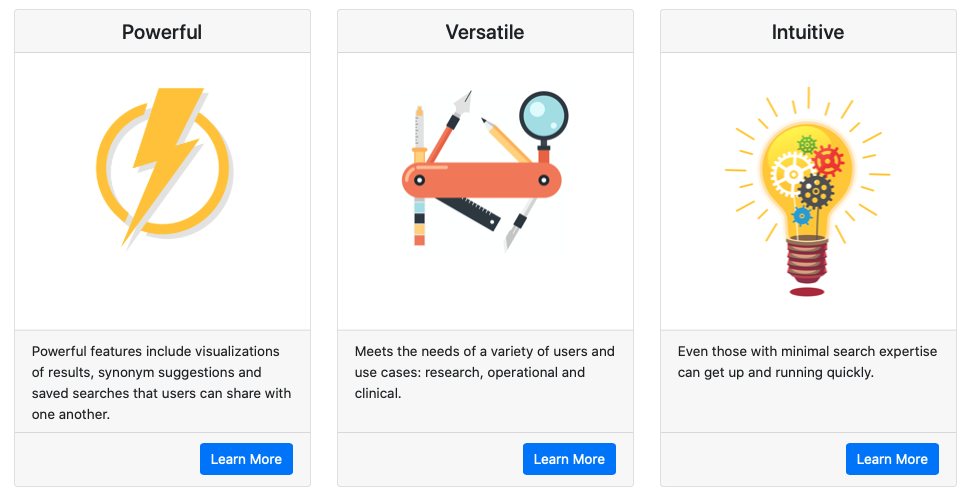
\includegraphics[width=0.8\textwidth]{Resources/Images/Banner4.png}
    \caption{Caption}
    \label{fig:my_label}
\end{figure}

%%%%%%%%%%%%%%%%%%%%%%%%%%%%%%%%%%%%%%%%%%%%%%%%%%%%%%%%%%%%%%%%%%%%%%%%%
% Example Sub-Figure with Sub-Captions                                  %
%%%%%%%%%%%%%%%%%%%%%%%%%%%%%%%%%%%%%%%%%%%%%%%%%%%%%%%%%%%%%%%%%%%%%%%%%
\begin{figure}
    \centering
    \begin{subfigure}{0.4\textwidth}
        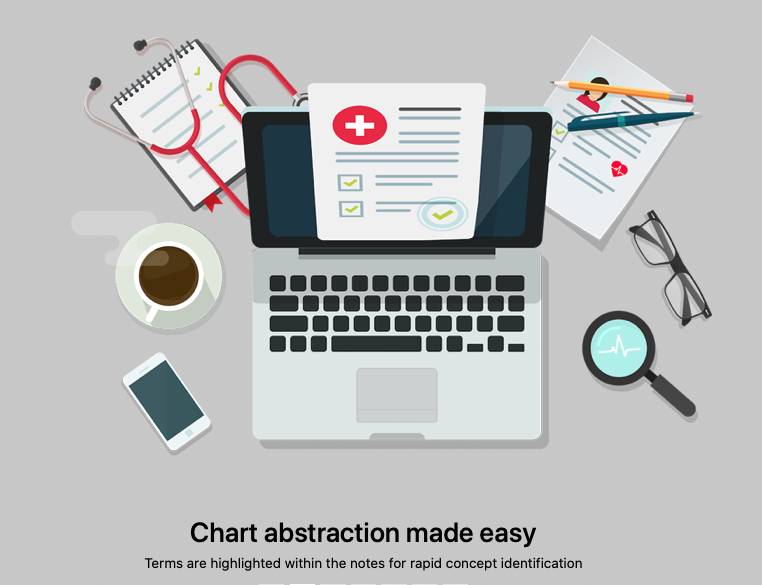
\includegraphics[width=\textwidth]{Resources/Images/Banner1.png}
        \caption[width=\textwidth]{Example Image 1}
        \label{fig:sub_bigrams3_apdx}
    \end{subfigure}
    \hfill
    \begin{subfigure}{0.4\textwidth}
        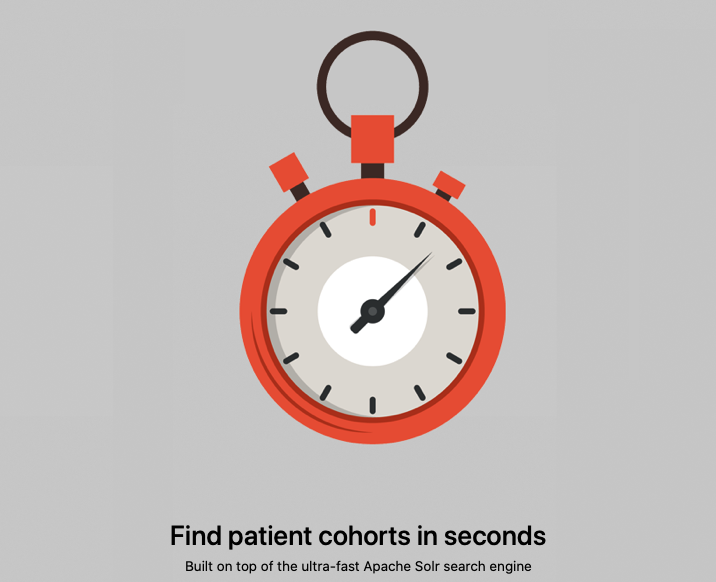
\includegraphics[width=\textwidth]{Resources/Images/Banner2.png}
        \caption[width=\textwidth]{Example Image 2}
        \label{fig:sub_trigrams3_apdx}
    \end{subfigure}
    \hfill
    \caption{Example multi-image figure}
    \label{fig:subfig_example}
\end{figure}

%%%%%%%%%%%%%%%%%%%%%%%%%%%%%%%%%%%%%%%%%%%%%%%%%%%%%%%%%%%%%%%%%%%%%%%%%
% Example Figure with Wrapped Text                                      %
%%%%%%%%%%%%%%%%%%%%%%%%%%%%%%%%%%%%%%%%%%%%%%%%%%%%%%%%%%%%%%%%%%%%%%%%%
\begin{wrapfigure}{L}{0.5\textwidth}
    \centering
    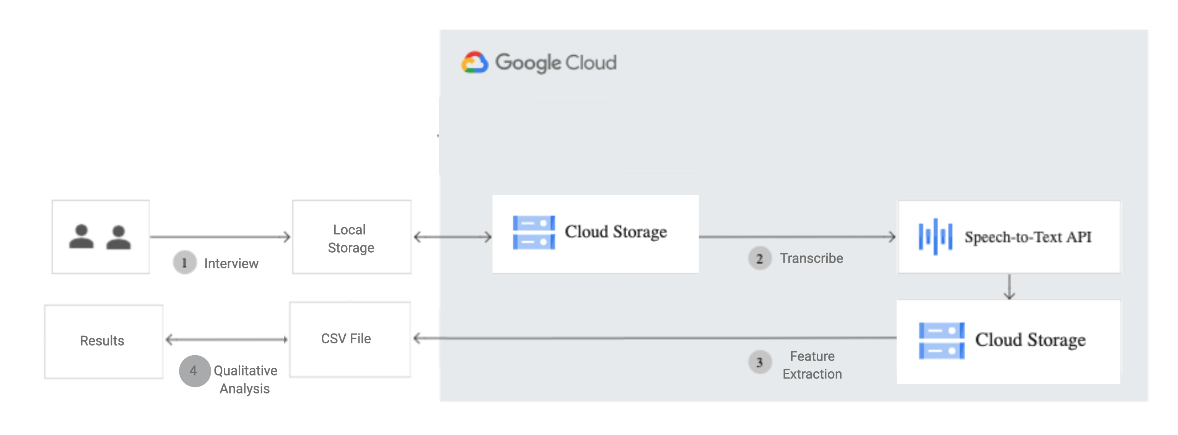
\includegraphics[width=0.45\textwidth]{Resources/Images/Workflow2.png}
    \caption{Example of figure that text will wrap around}
    \label{fig:UM_interview_wordcloud}
\end{wrapfigure}
\lipsum[1]
\lipsum[2]


\addtocontents{toc}{\protect\setcounter{tocdepth}{2}}

\chapter{Example Open Source Code Link}

% Appendix sections, subsections etc should not appear in the table of 
% contents. So set tocdepth to 0 and set it back to 2 at the end. Do 
% this for each appendix.
\addtocontents{toc}{\protect\setcounter{tocdepth}{0}}


\section{Repositories}
\label{sec:code_appendix}
Code for the transcription process in this project is open source and can be found at \url{https://github.com/colby-reyes/EMERSE}.
The EMERSE system is also open source. Its repository can be found here: \url{https://github.com/project-emerse}


\addtocontents{toc}{\protect\setcounter{tocdepth}{2}}
\chapter{EMERSE Information}

% Appendix sections, subsections etc should not appear in the table of 
% contents. So set tocdepth to 0 and set it back to 2 at the end. Do 
% this for each appendix.
\addtocontents{toc}{\protect\setcounter{tocdepth}{0}}

\section{Learn More About EMERSE}
\label{sec:emerse_info}


Though the EMERSE project is open-source, the projects here are private since we want to track the usage of it since it is grant-funded. If you want accesss, send the EMERSE team a message at \nolinkurl{EMERSE-team@umich.edu}.

\section{Contact}
\label{sec:emerse_contact}
Code for this project is open source and can be found at \url{https://github.com/colby-reyes/EMERSE}.


\addtocontents{toc}{\protect\setcounter{tocdepth}{2}}
\end{appendices}

\end{document}
